\section{Average Word-length analysis}
\subsection{First results}
After calculating and plotting the average word-length of all collections in the Pali canon, the following chart ensued:\\

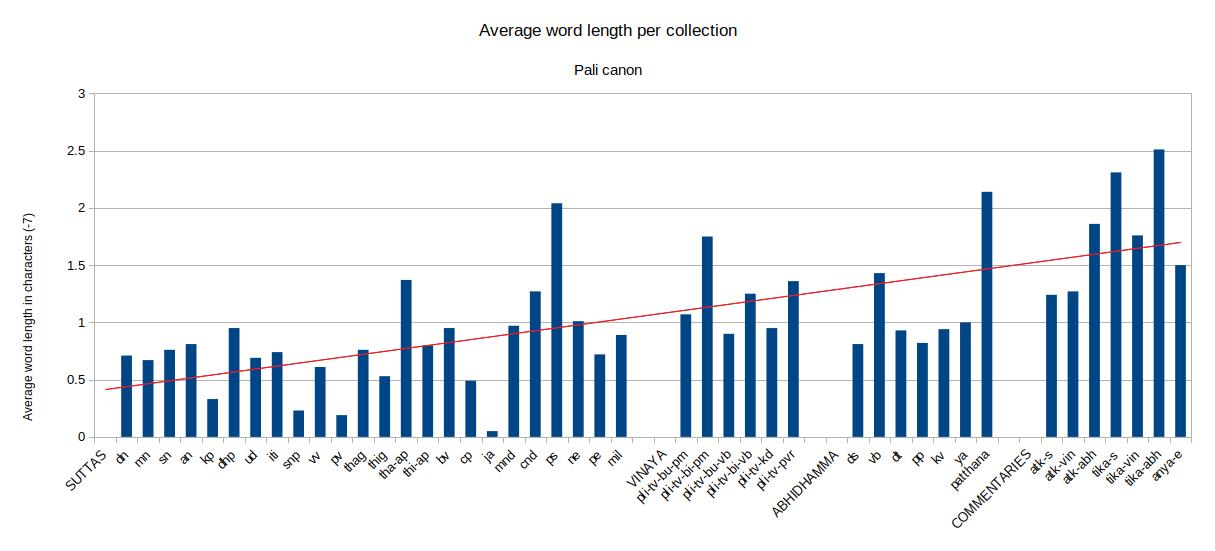
\includegraphics[width=\linewidth]{chart1.jpg}
\captionof{figure}{The average word-length in characters above 7 per book in the Pali canon. The red line shows the linear trendline (regression through equation y=a*x+b)}
\label{chart1}

\medskip
Some interesting things can be seen from this chart. First of all, it looks like those books that are generally accepted as "Early Buddhist" (see \citep{sujatobrahmali}) indeed have a lower average word-length while the later commentarial texts have a much higher average word-length.

The Vinaya and Abhidhamma texts as well as the later Sutta texts seem to all be in between with roughly the same average word-length, indicating that these texts might have developed at the same time.

However, there are also some books that do not seemingly match this broad pattern.

The first thing that struck me is the relative high value of the Dhammapada, which is generally seen as one of the earliest Buddhist texts. Then there are other discrepancies like the Jātaka and the Bhikkhuni Patimokkha. So I will explore these in more detail below.

\subsection{Dhammapada}
Analysing the Dhammapada (\url{https://suttacentral.net/dhp/pli/ms}), I noticed that especially the headings have a much larger word-length than the verses. 

If we keep in mind that all early texts were only transmitted orally and organized and written down at a much later date, it is quite possible that headings were inserted into the texts later.

So calculating the same chart with the headers taken out gives the following interesting picture:\\

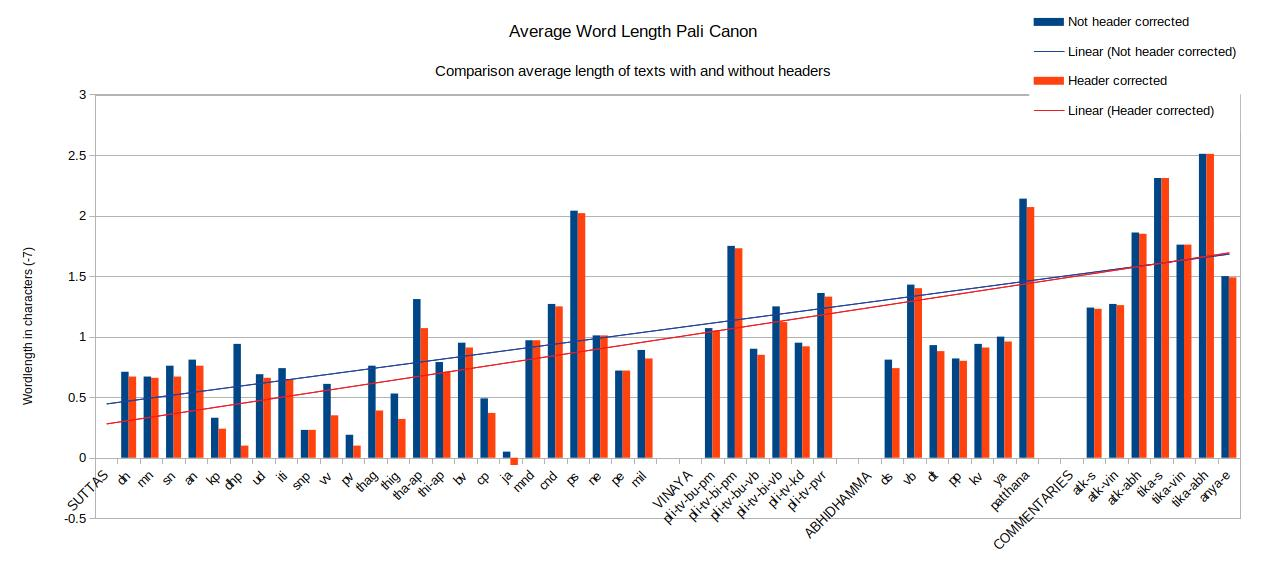
\includegraphics[width=\linewidth]{chart2.jpg}
\captionof{figure}{The average word-length in characters above 7 per book in the Pali canon comparing calculations with and without headers. The blue and red lines shows the linear trendlines resp. (regression through equation y=a*x+b)}
\label{chart2}

\medskip
Removing headers from the calculation and just analysing the prose or verse text suddenly gives a very different picture for expecially the Dhammapada, which has now jumped from a relatively high value to a much lower value which is much more in line with our accepted understanding of the Dhammapada as a very early text.

Another interesting thing we see in this chart is that removing the headers has a much more dramatic effect on the Early Buddhist texts and the commentarial texts are hardly affected. So I think it is safe to assume that headers are indeed inserted into the texts later.

\subsection{Anguttara Nikaya}
For comparison, the next chart shows the same data but with the 0-line at the level of the highest of the Early Buddhist books, which is the Anguttara Nikaya. The fact that the Anguttara Nikaya is the book with the highest average word-length is consistent with our understanding that of all the early Buddhist Nikayas, this book has had the most influence by later insertions. \\

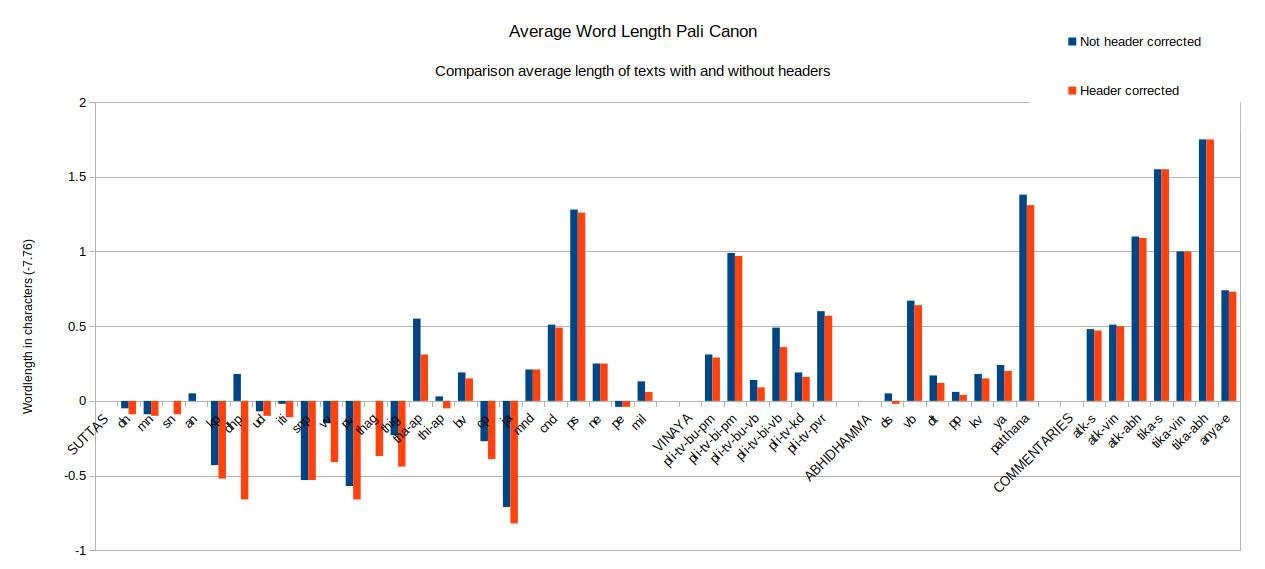
\includegraphics[width=\linewidth]{chart3.jpg}
\captionof{figure}{The average word-length in characters above 7.76 per book in the Pali canon comparing calculations with and without headers. The blue and red lines shows the linear trendlines resp. (regression through equation y=a*x+b)}
\label{chart3}

\subsection{Verse vs. prose}
When we look at the early Buddhist books, from the Digha Nikaya through to the Therigatha, we notice another interesting phenomenon: books with predominantly verses have a much lower average word-length than books with prose.

There are various ways in which this can be explained. First of all, it might be that verse, by its very nature, needs shorter words. But we will see in the analysis of the Jātaka that this is not always the case.

Another possibility is that due to the history of oral tradition, it was much easier to remember and recite verses than prose and we do indeed see that verse summaries of prose teachings were one method to ensure oral transmission.

\subsection{Bhikkhuni Patimokkha}
The average word-length of the Bhikkhuni Patimokkha seems very high in comparison to the other books of the Vinaya. This is not surprising if we remember that the Bhikkhuni Patimokkha had been lost and was actually reconstructed from a commentarial text. No doubt due to it's history, the text would also have acquired some of it's later use of the Pali language, most notably with concatted and therefore longer words. This does not say anything about the actual age of the original Bhikkhuni Patimokkha, only of the current version we have.

\subsection{Jātaka}
One of the most striking anomaly is the Jātaka collection. In fact, it is the collection with by far the lowest average word-length.

The Jātaka verses are verses are generally seen as pre-Buddhist tales. They came into the Buddhist canon, not only because the Buddha himself sometimes used these tales in his teachings, but more because the old tales would get a story woven around them in which these were said the stories of the Buddha's previous lives. However, these stories are not in the Mahāsaṅgīti Tipiṭaka version of the Jātaka, where only the verses are used. So it is maybe not so surprising that these stem from an earlier use of the Pali language and therefore have a shorter overall word-length.

The below figure shows the distribution of the Jātakas.\\

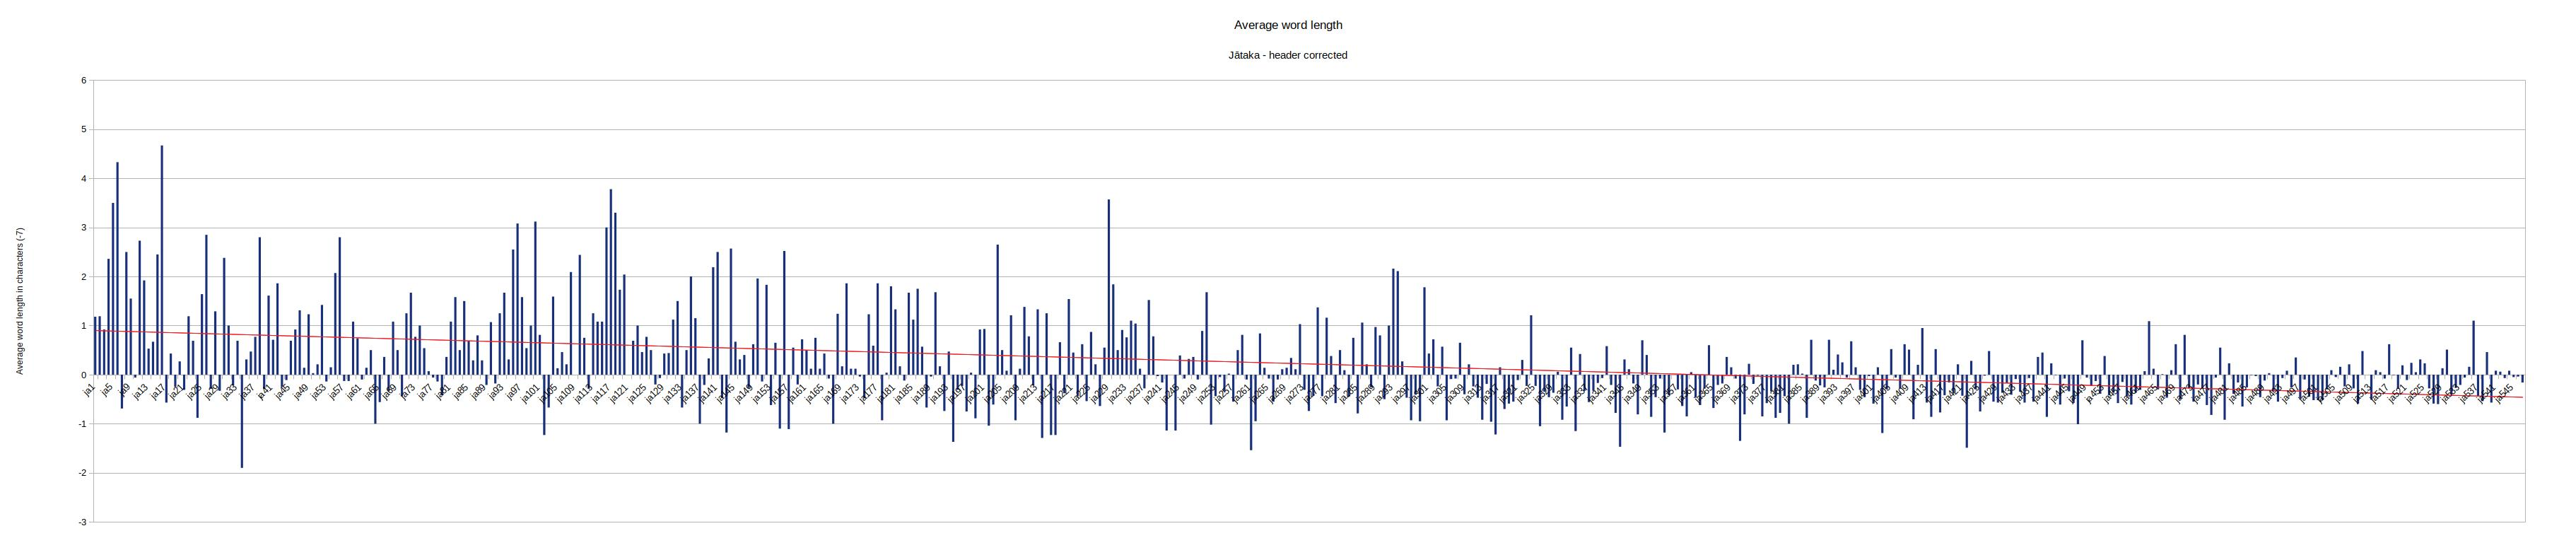
\includegraphics[width=\linewidth]{jataka.jpg}
\captionof{figure}{The average word-length in characters above 7 per book in the Pali canon comparing calculations with and without headers. The red line shows the linear trendline (regression through equation y=a*x+b)}
\label{jataka}

\medskip
This figure shows an interesting trend: the shorter Jātakas with a lower number seem to have a much higher word-length on average than the ones further in the collection. 

The next figure shows the number of parallels listed on SuttaCentral for the texts in this collection on a logarithmic scale. \\

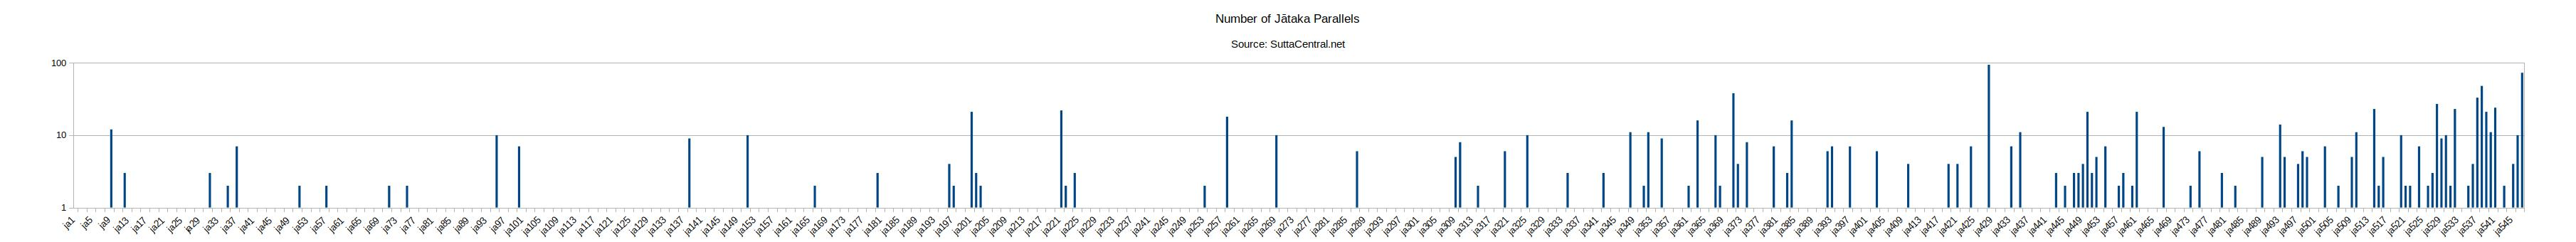
\includegraphics[width=\linewidth]{jatakapars.jpg}
\captionof{figure}{The number of parallels as listed on SuttaCentral on a logarithmic scale}
\label{jatakapars}

\medskip
Although there are not very many known parallels for many of these texts, it is clear from this that the most parallels appear in the higher end of the Jātaka collection.

From both of these charts it would seem that the Jātaka with a higher number are likely to be earlier than the first part of the collection. Of course we cannot make any assumptions about the lateness or earlyness of individual suttas based on this method, especially if many of these only contain just one verse, but it is an indication of a general trend.

Another interesting collection as is seen in figure \ref{chart3} is the Cariyāpiṭaka. A small collection of only 35 verse-texts, it mainly comprises of retellings of the Jātaka stories. Analysing this in a chart we get the following:\\

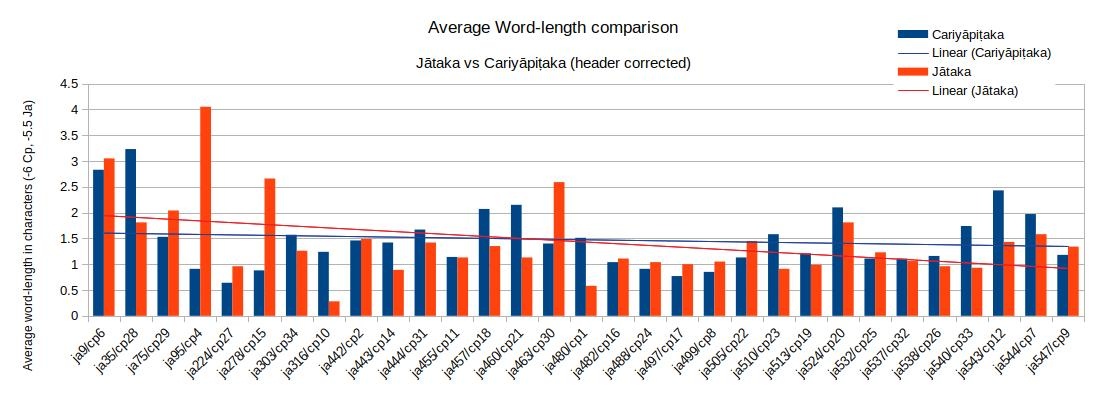
\includegraphics[width=\linewidth]{jacp.jpg}
\captionof{figure}{Comparison of Jātaka with Cariyāpiṭaka (Note that for the purpose of this comparison the value of length for Cariyāpiṭaka is .5 characters higher than for Jātaka)}
\label{jacp}

\medskip
There seems to be a rough, but not entirely convincing, similar trend between the two collections. More notably we see that most of the Cariyāpiṭaka are retellings of the Jātaka with higher numbers. This could be another indication that the latter part of the collection is earlier than the first part.
